\documentclass[11pt,a4paper,oneside]{article}
\usepackage[utf8]{inputenc}
\usepackage[french]{babel}
\usepackage[T1]{fontenc}
\usepackage{graphicx}
\usepackage{charter}
\usepackage{hyperref}
\usepackage[left=2cm,right=2cm,top=2cm,bottom=2cm]{geometry}
\author{Mylann Dupuy}
\title{Rapport de stage}
\begin{document}
\maketitle
\newpage
\tableofcontents
\newpage
\section{Contexte}
Le centre Jean Bernard / Clinique Victor Hugo voudrait mettre un nouveau système de déploiement pour déployer diverses logiciels.
\section{Objectif(s)}
L'objectif est de déployer les logiciels utilisés couramment et de les mettre à jour. Le système doit fonctionner avant la fin du stage. 
\subsection{Cahier des charges}
bla bla
\\
\subsection{Contraintes}
Lors du déploiement, les postes sont constamment utilisé par le personnel du centre. Pour pouvoir intervenir, il faut appelé la personne présente sur le poste et intervenir à distance avec \textbf{TightVNC}.
\subsection{Matériels disponible}
\begin{itemize}
	\item \textbf{1 Ordinateur} pour administrer et surveiller OCS.
	\item \textbf{1 Serveur virtuel} sous 	\textbf{Debian 8.7}.
	\item \textbf{1 Serveur de stockage}  pour l'accès aux exécutables prévus pour les scripts. 

\end{itemize}
\newpage
\section{Solutions}
\subsection{Comparaison}
En farfouillant sur Internet et aussi avec mes connaissances personnelles, j'ai recensé 5 solutions de déploiement mais dans notre contexte, il y a 2 solutions qui seront comparées \\ \\
%%%%%%%%%%%%%%%%%%%%%%%%%%%%%%%%%%%%%%%%%%%%%%%%%%%%%%%%%%%%%%%%%%%%%%%%%%%%%%%%%%%%%%%%%%%%%%%%%%%%%%%%%%%%%%%
\begin{tabular}{|p{3.1cm}|p{6.5cm}|p{6.5cm}|}
	\hline
	\centering Solutions : & \centering Avantages : & Inconvénients : \\
	\hline
	%%%%%%%%%%%%%%%%%%%%%%%%%%%%%%%%%%%%%%%%%%%%%%%%%%%%%%%%%%%%%%%%%%%%%%%%%%%%%%%%%%%%%%%%%%%%%%%%%%%%%%%%%%%
	\centering OCS Inventory NG  & \begin{itemize}
							\item Faible utilisation de la bande passante 
							\item Plugins pour GLPI							
							\item Supervision des logiciels installé
							\item Logiciel libre disponible sous Windows Server / Client
							\item Inventaire complet des postes							
						\end{itemize} & \begin{itemize}
												\item Wiki non à jour  
												\item Paquets Debian en version 2.0.5																			\end{itemize} \\
	\hline
	%%%%%%%%%%%%%%%%%%%%%%%%%%%%%%%%%%%%%%%%%%%%%%%%%%%%%%%%%%%%%%%%%%%%%%%%%%%%%%%%%%%%%%%%%%%%%%%%%%%%%%%%%%%
	\centering WAPT  & \begin{itemize}
							\item Automatisation d'installation, MAJ et suppressions logiciels 
							\item Centralisation graphique du déploiement
							\item Facilité pour les MAJ 
							\item Gestion des dépendances
							\item Logiciel libre													
						\end{itemize} & \begin{itemize}
												\item Configuration à faire pour faire cohabiter WSUS et WAPT 
												\item Packages propre à WAPT (.wapt)
												\item Suite Microsoft Office non Disponible
												\item Supervision des logiciels installé
												\item Création de paquets + ou - complèxe
												\item Certains logiciels ne sont plus à jour			
										\end{itemize} \\
	\hline	
\end{tabular}
%%%%%%%%%%%%%%%%%%%%%%%%%%%%%%%%%%%%%%%%%%%%%%%%%%%%%%%%%%%%%%%%%%%%%%%%%%%%%%%%%%%%%%%%%%%%%%%%%%%%%%%%%%%%%%
\\ \\
Nous avons décidés de mettre en place \textbf{OCS Inventory NG 2.3} (cf.références) car les logiciels qui doivent être déployer seront facilement mis à jour contrairement à WAPT.
\\
\subsection{Mise en \oe{}uvre}
\subsubsection{Avant de commencer} 
Nous avons créer une machine virtuelle sous Hyper-V (cf.références) en lui mettant comme ressources :\\ \begin{itemize}
				\item 1 image ISO de Debian 8.7
				\item 4 Go de mémoire vive
				\item 1 C{\oe}ur du processeur
				\item 50 Go d'espace disque
				\item 1 connexion au réseau CJB	
\end{itemize} 

\begin{center}
\textbf{Cette configuration est hébergée sur le poste de M.Deshayes}
\end{center}
\newpage
\subsubsection{Installation}
Lors de l'installation, j'ai tout laissé par défaut sauf le proxy qui à été renseigné. Suite à l'installation, j'ai eu à installer \textbf{openssh-server} pour tout faire via \textbf{PuTTY}.\\

Depuis SSH, il fallait installer un serveur Web, un serveur BDD, PHP, Perl et leurs modules (\textbf{apache2, mylsql-server, php5, perl, libxml-simple-perl, libcompress-zlib-perl, libdbi-perl libdbd-mysql-perl,libapache-dbi-perl, libnet-ip-perl, libsoap-lite-perl}). Pour les modules Perl en cas de problèmes de paquets, il faut les télécharger et les installer à la main depuis ce site \url{http://search.cpan.org/} \\

S'il manque des paquets, le script d'installation d'OCS Inventory les installera mais dans notre cas, on est derrière un proxy donc vaut mieux tout installer avant. \\

Pour installer OCS Inventory NG, j'ai utilisé l'archive qui était sur le site via \url{www.ocsinventory-ng.org/fr/} et la documentation non à jour via \url{http://wiki.ocsinventory-ng.org/index.php?title=Documentation:Server/fr}
\section{Principe de fonctionnement}
\begin{figure}[hbtp]
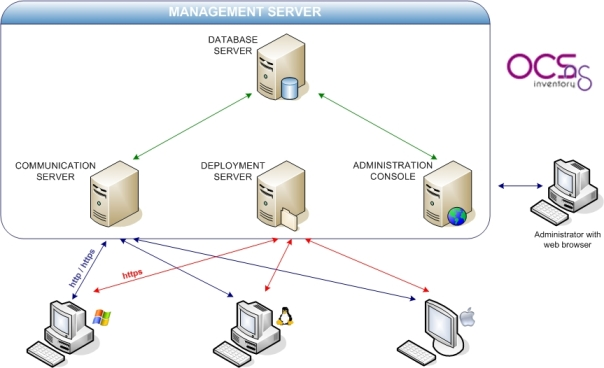
\includegraphics[scale=0.8]{../../../Downloads/deploy.jpg}
\caption{Schéma de déploiement}
\end{figure}


%Résumé d'utilisation d'OCS
% Utilisation du Module de déploiement
\subsection{Scripts utilisés}
bla bla
\section{Résultat Final}
bla bla
\subsection{Problèmes rencontrés}
bla bla
\section{Conclusion}
bla bla
\section{Annexes}

\section{Références}
Microsoft Hyper-V :
OCS Inventory NG 2.3 :
\end{document}